
\LARGE Manual de Instrucões.

		\begin{multicols}{2}
	
	\normalsize	De forma geral, o sistema é muito simples: um arquivo HTML é gerado em \LaTeX, e disponibilizado  numa página do servidor Apache local, e entao configuramos todos os computadores dos alunos, para que abram esta página automaticamente, através do navegador, logo na inicialização do seu Desktop Linux favorito, que também é inicializado automaticamente.
	
	É uma tarefa que pode ser realizada por qualquer técnico ou profissional de TI, que tenha acesso à senha root do sistema, alguns conhecimentos em redes, HTML, Apache, e saiba usar minimamente o terminal, habilidades mínimas para qualquer instrutor de Informática.
	
	Quanto à linguagem \LaTeX, você não terá dificuldades em aprender o básico, rápidamente.
	
	Desta forma, basta o Instrutor ligar os computadores e, e em poucos minutos, os alunos terão na tela um índice de todas as aulas e atividades, de todos  os bimestres, de todos os anos letivos, e o professor terá não somente um guia de aulas, mas todo o Universo que quiser criar em hipertexto, desde aulas expositivas, imagens, videos, jogos, simuladores espaciais, tudo o que é necessario para transformar aquilo que seria só mais uma aula chata, numa grande viagem de exploração pelo universo digital!
	
	E fazemos isso de forma simples, automática, rápida, eficiente, pedagogicamente correta, livre de pirataria e ainda sem custos adicionais para a Escola, pois todo o sistema é desenvolvido em Software Livre.
	
	As atividades escritas por mim, que constam neste documento, foram testadas ao longo de 10 anos, em sala de aula, em turmas de 15 a 20 alunos, de 6 a 15 anos, mas é cruxial lembrar que o BNCC permite que cada Escola, professor ou instrutor encontre sua própria metodologia, e desenvolva seu próprio roteiro de aulas, de acordo com as necessidades de cada turma ou Escola.
	
	Justamente por este motivo, este documento é liberado sob licença Creative Commons, em formato de código aberto: para que as aulas sejam editáveis por qualquer escola, professor ou instrutor que queira fazê-lo.
	
	Sinta-se a vontade para copiar, alterar e distribuir cópias, observando a licença Creative Commons Não Comercial.
	
	Um ano letivo tem aproximadamente 8 meses, com 4 aulas cada um. Ou seja, 32 aulas anuais, para cada ano de ensino. Se temos uma escola de 5 anos, resulta num total de 160 aulas, independente do número de alunos.
	
	Então são 160 arquivos em formato texto editaveis, um para cada aula.
	
	No \LaTeX, estes arquivos podem ser tanto um texto, como podem carregar imagens, ou ate uma biblioteca inteira de imagens, assim como links para diversas atividades, como aplicativos, programas, páginas web ou arquivos salvos na máquina local, ou mesmo no servidor externo.
	
	Utilizando \LaTeX, criamos um arquivo HTML, que pode ser lido em qualquer celular que esteja conectado à rede local da escola, propiciando ainda mobilidade ao professor, ja que também pode leva-lo para casa, no formato PDF.
	
	Este mesmo PDF e transformado em formato HTML, através de um script simples.
	
	%Para isso, primeiro e necessario instalar o pacote poppler-utils:
	%
	%\begin{lstlisting}
	%	apt install poppler-utils
	%\end{lstlisting}
	
	Então, basta converter o arquivo:
	
	\begin{lstlisting}
		pdf2htmlEX PROJETO.pdf index.html
		
		pdftohtml [options] [pdf source file] [html output file]
		
		pdftohtml -v PROJETO.pdf index.html
	\end{lstlisting}
	
	
	O HTML resultante vai para a página Apache do servidor local, e todos os outros computadores são direcionados a ela, na inicialização.
	
	Para fazê-lo, primeiro precisamos configurar todos os computadores, comecemos pelo terminal:
	
	\textit{Alt+F2 == xterm}
	
	\begin{lstlisting}
sudo passwd root\\
(digite 2x a nova senha de root)
		
su -\\
Password:
		
apt update
		
apt -f install openssh-server openssh-client apache tomcat9 arduino frozen-bubble debian-junior gcompriz...
		
chown -vR professor /var/lib/tomcat9/webapps/ROOT/index.html
		
chown -vR professor /var/www/html/index.html
	\end{lstlisting}
	
	\begin{lstlisting}
pdf2htmlEX PROJETO.pdf index.html
		
cp -v index.html /var/lib/tomcat9/webapps/ROOT/index.html
		
cp -v index.html /var/www/html/index.html
	\end{lstlisting}
	
\end{multicols}



%SHELL
% Template for documenting your Arduino projects
% Author:   Luis Jose Salazar-Serrano
%           totesalaz@gmail.com / luis-jose.salazar@icfo.es
%           http://opensourcelab.salazarserrano.com

%%%%% Template based in the template created by Karol Koziol (mail@karol-koziol.net)

%\linespread{1.3}
\lstdefinestyle{C}{
	language=sh,
	fillcolor=\color{white},
	backgroundcolor=\color{white},
	basicstyle=\small\ttfamily,
	breakatwhitespace=false,
	breaklines=true,
	captionpos=b,
	commentstyle=\color{gray},
	deletekeywords={...},
	escapeinside={\%*}{*)},
	extendedchars=true,
	frame=single,
	keepspaces=true,
	keywordstyle=\bfseries\color{orange},
	morekeywords={*,...},
	numbers=left,
	numbersep=2mm,
	numberstyle=\footnotesize\color{darkgray},
	rulecolor=\color{black},
	rulesepcolor=\color{black},
	showspaces=false,
	showstringspaces=false,
	showtabs=false,
	stepnumber=1,
	stringstyle=\color{orange},
	tabsize=3,
	title=\lstname,
	emphstyle=\bfseries\color{blue},
	framexleftmargin=0mm,
	framextopmargin=1mm
}


\begin{multicols}{2}
	\normalsize
	
	Supondo que você sabe instalar um sistema operacional GNU de Kernel Linux, sugerimos utilizar uma distribuição baseada em Debian, Ubuntu, ou, de preferência um a distro especializada em educação, como Linux Educacional, Zorin.
	
	Ubuntu Studio revelou-se uma distribuição uma distribuição muito leve, estável e customizável.
	
	Distribuicões que utilizam Desktops mais leves, como Xubuntu ou Lubuntu, são indicadas para computadores mais antigos, de forma a aproveitar melhor os recursos de memória e processamento.
	
	Escolhida a distribuição, a primeira coisa a fazer é, óbviamente, instalar o sistema operacional, criando um usuário \textit{professor}, com privilégios de \textit{sudoer} ou \textit{admin}.
	
	Feito isto, instalado o sistema \textit{default}, vamos trocar a senha de \textit{root}, para facilitar nosso trabalho.
	
	No computador central do Laboratório (servidor, escolha aquele que tiver mais poder de processamento e memória, pois é nele que você vai passar os próximos anos da sua vida):
	
	Acesse sua área de trabalho, com a senha de usuário administrador (usuário "professor", criada durante a instalação), e abra o terminal, utilizando o atalho Alt+F2.
	
	Na caixa que aparecer na tela, digite \textit{xterm} ou \textbf{terminal}, e aperte Enter.
	
	A próxima janela é o terminal, não precisa ter medo dele! Na verdade, com o tempo, você vai passar a gostar muito dele!
	
	Digite no terminal, nesta ordem:
	
	\begin{lstlisting}
		sudo passwd root
		 Aperte Enter
	 Digite a nova senha
		 Aperte Enter (de novo)
		 Digite a nova senha (de novo)
		 Aperte Enter (demais uma vez)
	\end{lstlisting}
	
	Repare que, ao digitar a senha, nenhum caractere é escrito no terminal. Isto serve para proteger a nova senha de olhares maliciosos.
	
	Pronto. Agora você é ROOT, tem poderes supremos sobre a máquina.
	
	Por enquanto, vamos nos divertir com os novos super-poderes. Digite:
	
	\begin{lstlisting}
		su -
	\end{lstlisting}
	
	Aperte Enter, digite sua senha de \textit{root} e confirme, apertando ENTER.
	
	Ótimo, agora você tem controle total do servidor!
	
\textbf{Bem vindo ao mundo Linux, Padawan!}
	
Lembre-se, daqui por diante: \textbf{com grandes poderes, grandes responsabilidades você terá}!
	
	O próximo passo é instalar todos os aplicativos didáticos que os alunos utilizarão, bem como todas as ferramentas administrativas e protocolos de rede. Este script deve ajudá-lo:
	
	\begin{lstlisting}
		apt update
		apt install openssh-server openssh-client apache tomcat9 arduino frozen-bubble debian-junior gcompriz mc synaptic libreoffice -y
	\end{lstlisting}
	
	Reinicie o servidor, afim de que todos os novos serviços e protocolos instalados sejam carregados corretamente.
	
	Repita esta operação em \textbf{todos os computadores, de todos os alunos}.
	
	Segue o link para o github do projeto (\textbf{revisar}):
\end{multicols}

\begin{center}
	\Huge	\href{https://github.com/aravecchia/EFESTUS}{https://github.com/aravecchia/EFESTUS}
\end{center}

\vfill\null
\pagebreak

\begin{multicols}{2}
\Large Conhecimentos necessarios:
%
%txt $\rightarrow$ tex $\rightarrow$ html $\rightarrow$ apache $\rightarrow$ crontab $\rightarrow$ firefox $\rightarrow$ localhost $\rightarrow$ ssh


	\large
	\begin{itemize}
		\item Shell
		\item \LaTeX
		\item HTML
		\item Apache
		
		\vfill \null
		\columnbreak
		
		\Large Conhecimentos desejaveis:
		
		\item Python
		\item Eletrônica
		\item Arduino
	\end{itemize}
	
\end{multicols}
	\vfill \null
	\pagebreak

\begin{center}
	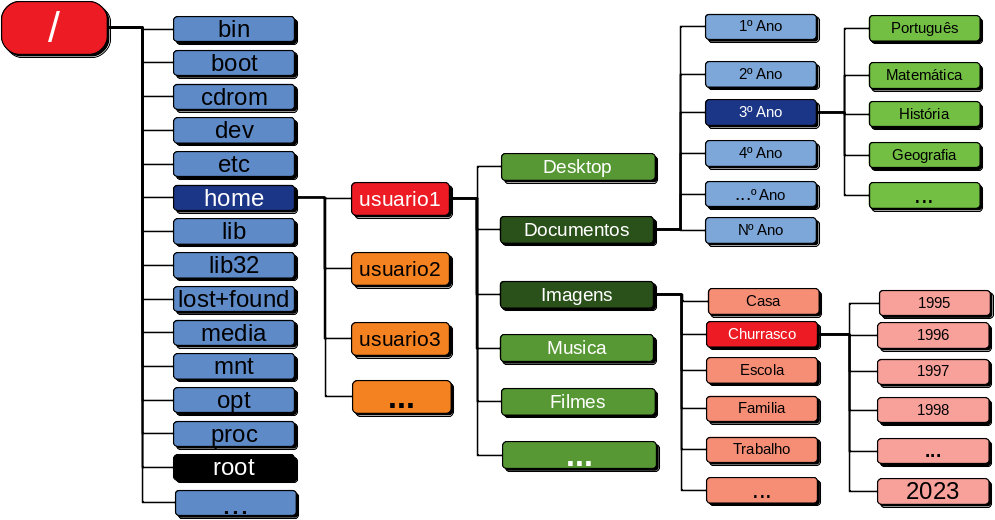
\includegraphics[height=\textheight]{./IMG-GIT/SVG/DIAGRAMAS.png}
\end{center}
\pagebreak

\begin{center}
	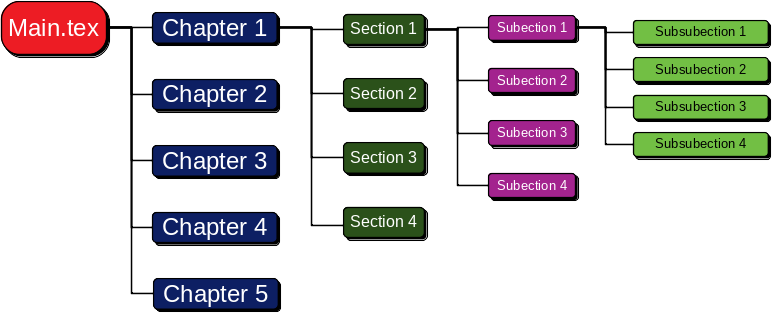
\includegraphics[width=\linewidth]{./IMG-GIT/SVG/DIAGRAMAS2.png}
\end{center}
\pagebreak


\begin{center}
	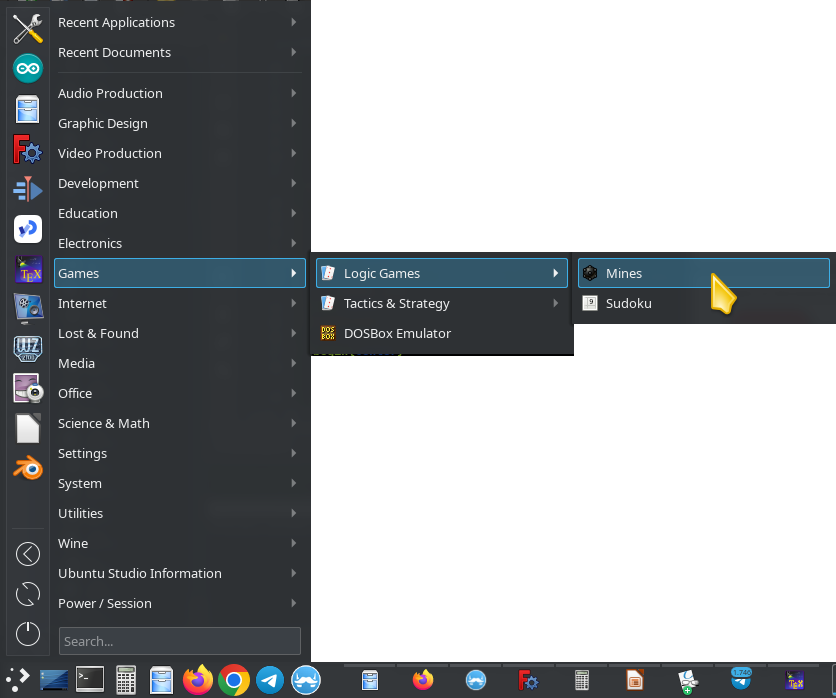
\includegraphics[height=\textheight]{./IMG-GIT/menu.png}
\end{center}
\pagebreak

{\Huge \LaTeX}
\begin{center}
	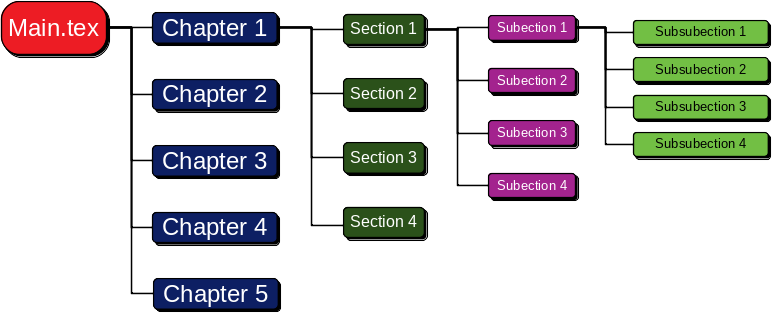
\includegraphics[width=\linewidth]{./IMG-GIT/SVG/DIAGRAMAS2.png}
\end{center}
\pagebreak

\begin{center}
	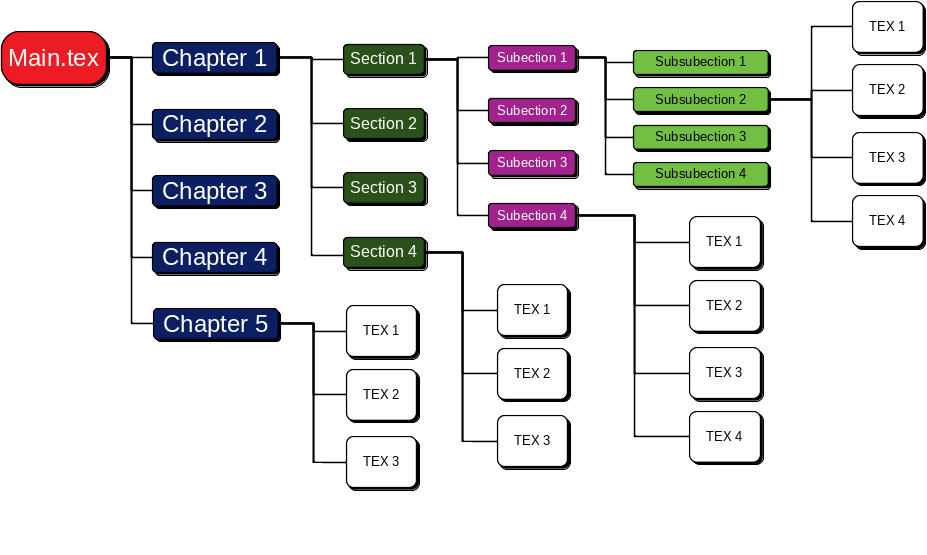
\includegraphics[height=\textheight]{./IMG-GIT/SVG/DIAGRAMAS3.png}
\end{center}
\pagebreak

\begin{center}
	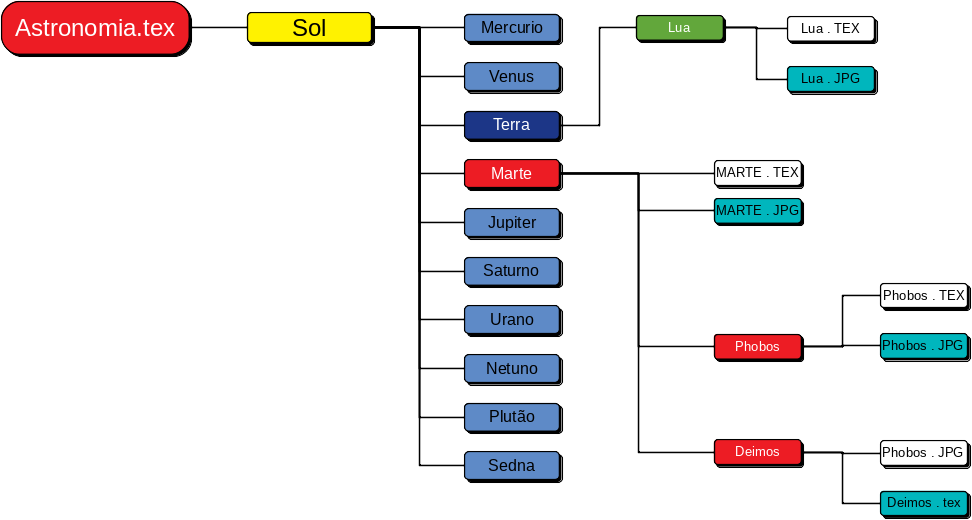
\includegraphics[height=\textheight]{./IMG-GIT/SVG/DIAGRAMAS4.png}
\end{center}
\pagebreak

\begin{center}
	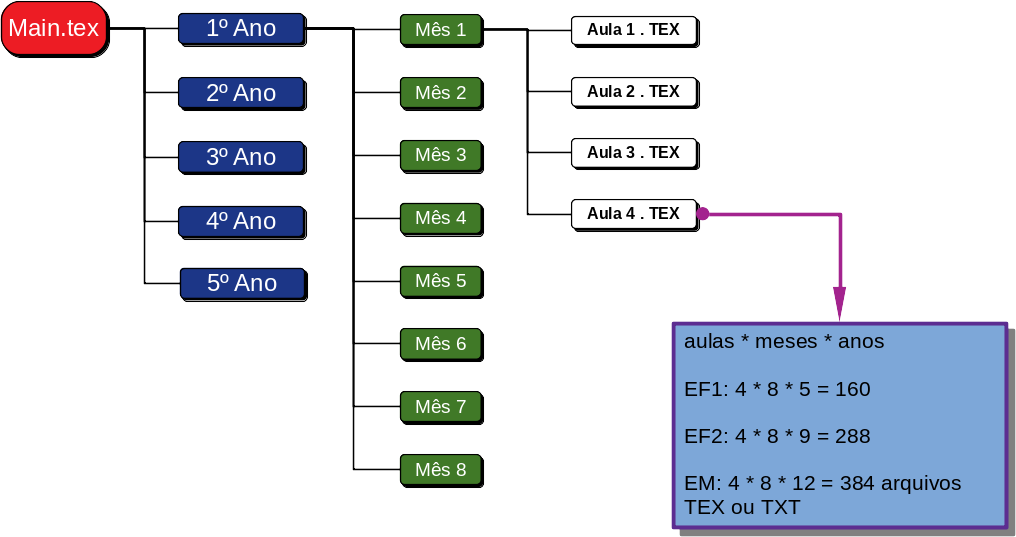
\includegraphics[height=\textheight]{./IMG-GIT/SVG/DIAGRAMAS5.png}
\end{center}
\pagebreak

\begin{center}
	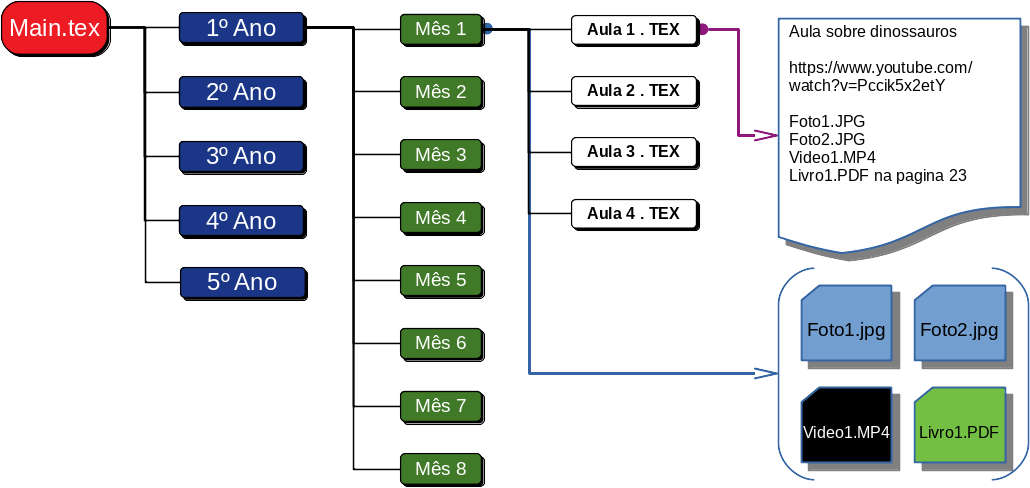
\includegraphics[width=\linewidth]{./IMG-GIT/SVG/DIAGRAMAS6.png}
\end{center}
\pagebreak


\begin{center}
	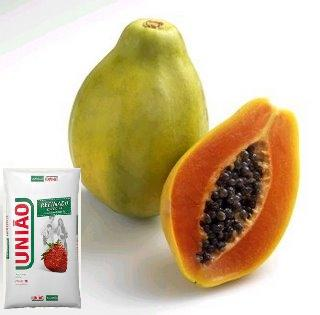
\includegraphics[height=\textheight]{./IMG-GIT/mamao.jpg}
\end{center}
\pagebreak

\begin{multicols}{2}
	\LARGE	 \textbf{Coisas que não vao acontecer}:
	
	\vspace*{10mm}
	\Large \textbf{Querido instrutor}:
	\large
	\begin{itemize}
		\item Quero um video sobre \nobreak dinossauros.
		
		\item Qual video, 'fessora?
		
		\item Não sei, coloca qualquer um.
		
		\item \textbf{Depois}: Mas não foi isso que eu pedi!
		
		\item Esse video não tem nada a ver com o projeto pedagógico da escola...
		
	\end{itemize}
	\vfill\null
	\columnbreak
	
	\begin{center}
		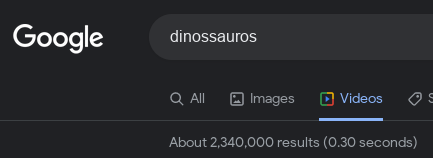
\includegraphics[width=\linewidth]{./IMG-GIT/dinossauros.png}
	\end{center}
	
	\textbf{Link}:
	\large
	\begin{itemize}
		\item https://www.youtube.com/watch?v=Pccik5x2etY
		\item \verb|\href{URL}{Dinossauros}|
		\item \href{https://www.youtube.com/watch?v=Pccik5x2etY}{Dinossauros}
	\end{itemize}
	
	
	\vfill\null
	\columnbreak
	
	\begin{center}5
		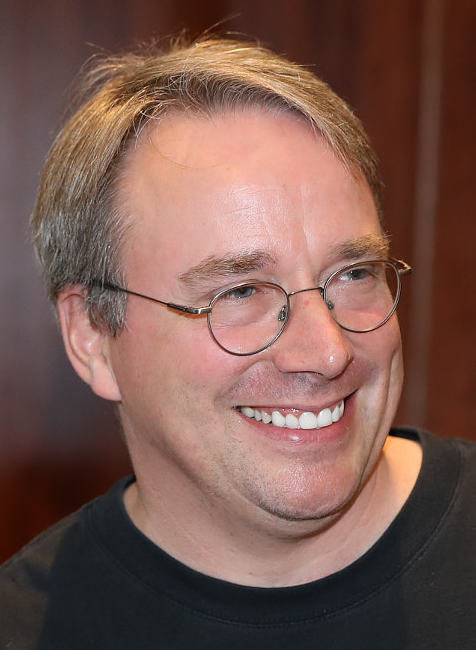
\includegraphics[height=.8\textheight]{./IMG-GIT/linus.jpeg}
	\end{center}
	
	\columnbreak
	\Large \textbf{AULAS que não vao acontecer}:
	
	\vspace*{5mm}
	
	\Large S. Alexandre, preciso fazer uma \nobreak atividade no Word:
	
	\large
	\begin{itemize}
		\item Baixar uma imagem do Google.
		\item Importar para um documento.
		\item Escrever um texto no Frontwork.
		\item Salvar o documento.
		\item Imprimir.
		\item Criancas de 9 anos, iniciantes.
		\item \textbf{50 minutos}.
	\end{itemize}
	
	%Com um tema, d ́a-se maior sentido a inser ̧c ̃ao de se ̧c ̃oes, pois al ́em de serem destacadas nos slides, podemos
	%transitar de uma para outra conforme queiramos.
	%2.5 Organiza ̧c ̃ao das informa ̧c ̃oes na lˆamina
	%A partir dos temas, podemos come ̧car a trabalhar com outras ferramentas importantes para a organiza ̧c ̃ao da
	%apresenta ̧c ̃ao.
	%2.5.1 Blocos
	%Um recurso interessante de organiza ̧c ̃ao de informa ̧c ̃oes  ́e a cria ̧c ̃ao de blocos dentro dos frames, o qual permite
	%criar um conjunto de informa ̧c ̃oes separadas com um t ́ıtulo. Isto  ́e feito atrav ́es dos seguintes comandos:
	%\frame{
		%	\begin{block}{T ́ıtulo do bloco}
			%		...
			%	\end{block}
		%	Estes blocos ser ̃ao separados em caixas que, na lˆamina, aparecer ̃ao em destaque.
		%	Exemplo 8 Utilizando o preˆambulo que foi constru ́ıdo no Exemplo 7, vamos inserir dois blocos em um frame.
		%	\begin{document}
			%		\frame{
				%			\frametitle{Exemplo 8}
				%			\begin{block}{Exemplo de bloco 1}
					%				Aqui escrevemos o texto do bloco 1.
					%			\end{block}
				%			\begin{block}{Exemplo de bloco 2}
					%				Aqui escrevemos o texto do bloco 2.
					%			\end{block}
				%		}

			\vfill \null
			\columnbreak
			
			\begin{center}
%				\vspace{20mm}
				\resizebox{\linewidth}{.3\textheight}{\color{black}\textbf{404}}
				\\
				\vspace*{5mm}
				{\Huge Aula não encontrada}
			\end{center}

	\vfill\null
	\columnbreak
	
	\begin{itemize}
				\item Pagina offline
				\item Sistema desatualizado ou incompatível
				\item Eu peguei no site do MEC, procura lá...
				\item É um video que tem o dinossauro subindo a montanha pra beber água numa cachoeira...
				\item Tá aqui no livro...
				\item Quando chegar o dia a gente vê...
				\item \textbf{Me ajuda, eu tô desesperado(a)!}
				\item \textbf{Eu não sei o que é pra fazer...}
			\end{itemize}
			
		\end{multicols}
	
			
	\vfill
	\pagebreak
		
		\vspace*{30mm}
	\begin{center}
			{\Huge \color{blue} Se a atividade não for programada, não tem atividade!}
	\end{center}
		
		\vfill\null
		\pagebreak
		
		\begin{center}
			
\includegraphics[height=.7\textheight]{./IMG-GIT/anjo.jpg}
			
			\resizebox{\linewidth}{20mm}{\color{magenta}\textbf{Não tem aula de Informática!}}
			
		\end{center}
		\vfill
		\pagebreak
		
		\ThisCenterWallPaper{1.2}{./IMG-GIT/enchente.jpg}
		\begin{center}
			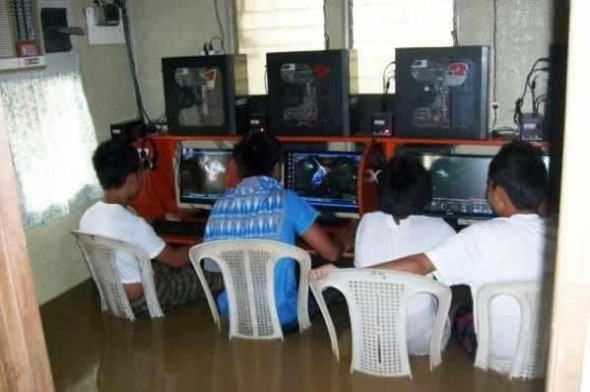
\includegraphics[height=.9\textheight]{./IMG-GIT/enchente.jpg}
		\end{center}
		
		\vfill
		\pagebreak
		
		\begin{frame}
			
			\centering % Para centralizarmos o vídeo
			\includemedia[
			label=nome-qualquer, % ! Importante para linkar o vídeo ao botao (ver abaixo)
			width=0.8\linewidth, height=0.5\linewidth, % Dimensões
			addresource=./MP4-GIT/VOGON.mp4, % ESTE É O SEU ARQUIVO DE VÍDEO (mesmo dir.)
			transparent, % Opcões para que o player tenha transparência
			activate=pageopen, % Se você deseja que o vídeo esteja "carregado" ao abrir a página
			flashvars={
				source=./MP4-GIT/VOGON.mp4
				&loop=false % Se você quer que o vídeo repita automaticamente 
				&scaleMode=letterbox % Manter proporcões (dimensionais) do vídeo
			}
			]{}{./MP4-GIT/VOGON.mp4}
			\vspace{1cm} % Espacamento entre vídeo e botao
			
			% Agora, você cria o botao para dar play/pause. Neste caso, o botao e apenas a letra "pi".
			
			%	\mediabutton[
			%	mediacommand=nome_qualquer:playPause,
			%	overface=\color{black}{{\strut $\pi$}},
			%	downface=\color{gray}{{\strut $\pi$}}
			%	]{{\strut $\pi$}}
			
			
		\end{frame}
		
		\vfill
		\pagebreak
		
		
		\begin{multicols}{3}	
			\begin{center}
				
\includegraphics[height=.5\textheight]{./IMG-GIT/fada.jpeg}
			\end{center}
			\begin{flushright}
				
\includegraphics[height=15mm]{./IMG-GIT/whatsapp.png}
			\end{flushright}
			
			\vfill	
			\columnbreak
			
			\begin{center}
				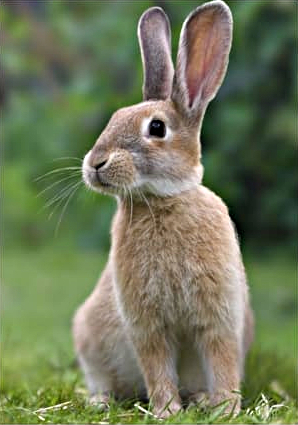
\includegraphics[height=.5\textheight]{./IMG-GIT/coelhinho.jpeg}
			\end{center}
			\begin{flushright}
				
\includegraphics[height=15mm]{./IMG-GIT/whatsapp.png}
			\end{flushright}
			
			\vfill	
			\columnbreak
			
			\begin{center}
				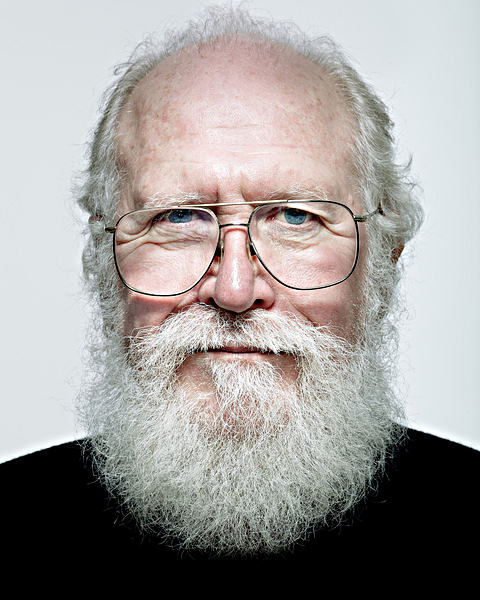
\includegraphics[height=.5\textheight]{./IMG-GIT/maddog.jpg}
			\end{center}
			\begin{flushright}
				
\includegraphics[height=15mm]{./IMG-GIT/whatsapp.png}
			\end{flushright}
		\end{multicols}	
		
		\vfill
		\pagebreak
		
		\begin{center}
			
\includegraphics[height=.7\textheight]{./IMG-GIT/anjo.jpg}
			
			\resizebox{.8\linewidth}{25mm}{\color{magenta}\textbf{É fácil!}}
			
		\end{center}
		\vfill
		\pagebreak
		
		\begin{center}
			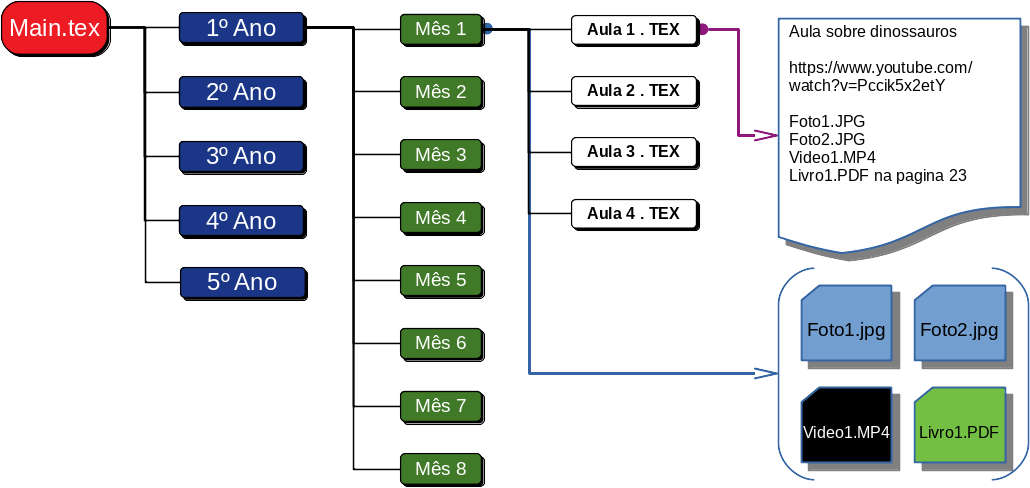
\includegraphics[width=\linewidth]{./IMG-GIT/SVG/DIAGRAMAS6.png}
		\end{center}
		\pagebreak
		
		\begin{center}
			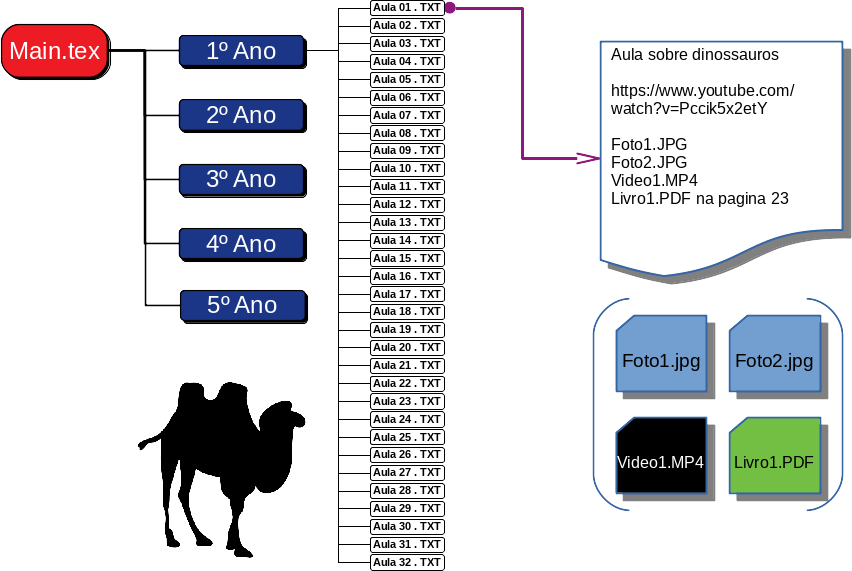
\includegraphics[height=\textheight]{./IMG-GIT/SVG/DIAGRAMAS7.png}
		\end{center}
		\pagebreak
		
		\begin{center}
			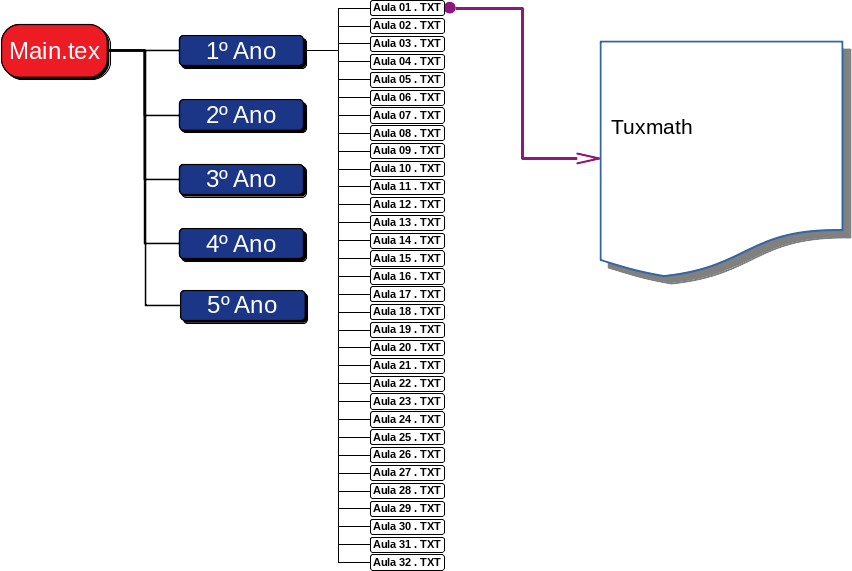
\includegraphics[height=\textheight]{./IMG-GIT/SVG/DIAGRAMAS8.png}
		\end{center}
		\pagebreak
		
		\begin{center}
			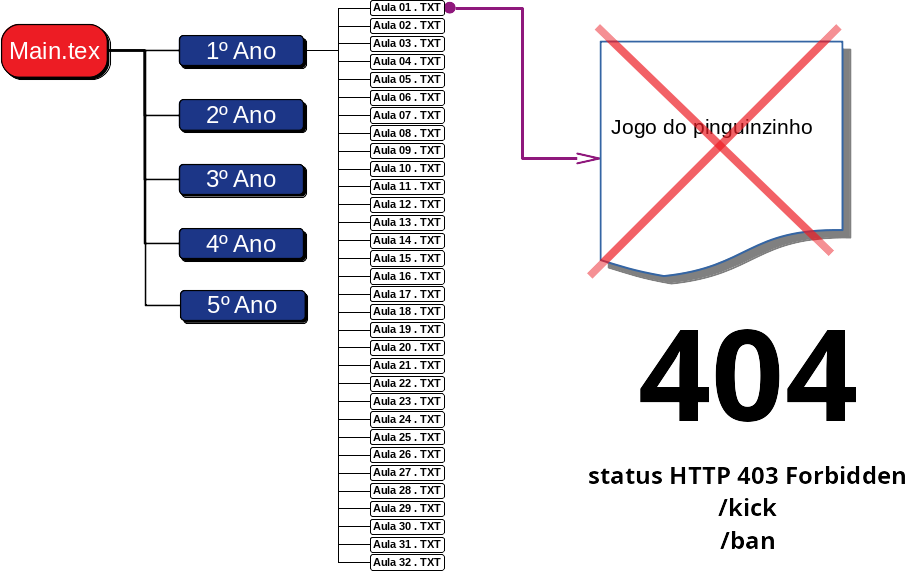
\includegraphics[height=.\textheight]{./IMG-GIT/SVG/DIAGRAMAS9.png}
		\end{center}
		
		\null
		\pagebreak
